\author{Łukasz Ziobroń}
\title[Crisis]{(R)evolution of C++}
\institute{lukasz@ziobron.net \and \url{http://ziobron.net}}
\date{code::dive, 2016-11-15}
\subject{Computer Science}
\subtitle{The Ultimate Hitchhiker's Guide to the C++}
%\logo{}

\begin{frame}
\titlepage
\end{frame}

\begin{frame}
  \frametitle{(R)evolution of JS}
  \centering 
  
\includegraphics[height=0.8\paperheight]{writing-device-drivers-with-js}
\end{frame}

\begin{frame}
  \frametitle{About the author}
  
\includegraphics[height=50pt]{html4-logo}
  
\includegraphics[height=40pt]{php-logo}
  
\includegraphics[height=60pt]{c++-logo}
\end{frame}


\slide{Key messages}{
  \begin{enumerate}
    \item C++ had a clear aim, which made it popular: to organize code better without the loss of efficiency
    \item C++ is even more popular now, because of new standards: C++11 and C++14.
    \item C++ will be one of the most popular programming languages in future so it's worth to invest your time and/or money to learn it.
  \end{enumerate}
}

\slide{Agenda}{
  \tableofcontents
}

\sectionSlide{Birth and evolution of C++}{c++-logo}{\paperheight}

\slide{Simula}{
    Simple program in Simula
}

\slide{BCPL}{
    Before C Programming Language\\
    \pause
    Basic Combined Programming Language
}

\slide{Genealogy}{
    Genealogy of C++ from C and Simula
}

\slide{Timeline}{
    Timeline on the bottom of page, new dates will gradually appear\\
    Maybe new type of slides? TimelineSlide?
}

\slide{C with Classes}{
\begin{itemize}%[<+->]
    \item classes
    \item derived classes
    \item public and private access control
    \item constructors and destructors
    \item \textbf<2>{call and return functions (removed later)}
    \item friend classes
    \item type checking and conversion of function arguments
\end{itemize}
}

\slide{Example code in C with Classes}{
    \lstinputlisting{"src/c-with-classes.hpp"}
}

\timelineSlide{LOL}{
    lol
}{
\newcommand{\foo}{\color{blue}\makebox[0pt]{{\large \textbullet}}\hskip-0.5pt\vrule width 1pt\hspace{\labelsep}}
\begin{table}
%    \renewcommand\arraystretch{1.4}\arrayrulecolor{blue}
%    \captionsetup{singlelinecheck=false, font=blue, labelfont=sc, labelsep=quad}
%    \caption{Timeline}\vskip -1.5ex
    \begin{tabular}{@{\,}r <{\hskip 2pt} !{\foo} >{\raggedright\arraybackslash}p{2.6cm}}
%        \toprule
%        \addlinespace[1.5ex]
        \textbf{1979} & \textbf{C with Classes}\\
        1981 & New features\\
        1983 & 1st std lib\\
        1984 & C84/C++\\
        1985 & Cfront 1.0\\
        1989 & Cfront 2.0\\
        1991 & Cfront 3.0\\
        1993 & Cfront 4.0\\
        1998 & C++98\\
        2003 & C++03\\
        2011 & C++11\\
        2014 & C++14\\
        2017 & C++17\\
        2020 & C++20\\
    \end{tabular}
\end{table}
}

\timelineSlide{C with Classes in 1981}{
    \begin{itemize}
        \item inline functions
        \item default arguments
        \item overloading of the assignment operator
    \end{itemize}
}{
    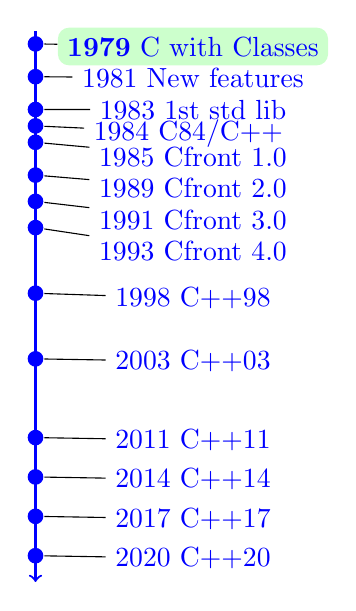
\begin{tikzpicture}
        \draw[thick,->,blue] (0,0.2)--(0,-6.8) % x axis
            node(1979)[pos=1/42,fill,circle,inner sep=2pt]{}
            node(1981)[pos=3.5/42,fill,circle,inner sep=2pt]{}
            node(1983)[pos=6/42,fill,circle,inner sep=2pt]{}
            node(1984)[pos=7.25/42,fill,circle,inner sep=2pt]{}
            node(1985)[pos=8.5/42,fill,circle,inner sep=2pt]{}
%            node(1986)[pos=8/42,fill,circle,inner sep=2pt]{}
%            node(1987)[pos=9/42,fill,circle,inner sep=2pt]{}
            node(1989)[pos=11/42,fill,circle,inner sep=2pt]{}
%            node(1990)[pos=12/42,fill,circle,inner sep=2pt]{}
            node(1991)[pos=13/42,fill,circle,inner sep=2pt]{}
            node(1993)[pos=15/42,fill,circle,inner sep=2pt]{}
            node(1998)[pos=20/42,fill,circle,inner sep=2pt]{}
            node(2003)[pos=25/42,fill,circle,inner sep=2pt]{}
            node(2011)[pos=31/42,fill,circle,inner sep=2pt]{}
            node(2014)[pos=34/42,fill,circle,inner sep=2pt]{}
            node(2017)[pos=37/42,fill,circle,inner sep=2pt]{}
            node(2020)[pos=40/42,fill,circle,inner sep=2pt]{};
            
        \draw[thin,blue]
            (2, 0) node(l1979)[fill=green!20,rounded corners] {\textbf{1979} C with Classes}
            (2,-0.4) node(l1981)[align=left] {1981 New features}
            (2,-0.8) node(l1983)[align=left] {1983 1st std lib}
            (2,-1.1) node(l1984)[align=left] {1984 C84/C++ }
            (2,-1.4) node(l1985)[align=left] {1985 Cfront 1.0}
%            (2,-2.0) node(l1986)[align=left] {1986 Cfront 1.1}
%            (2,-2.4) node(l1987)[align=left] {1987 Cfront 1.2}
            (2,-1.8) node(l1989)[align=left] {1989 Cfront 2.0}
%            (2,-3.2) node(l1990)[align=left] {1990 Cfront 2.1}
            (2,-2.2) node(l1991)[align=left] {1991 Cfront 3.0}
            (2,-2.6) node(l1993)[align=left] {1993 Cfront 4.0}
            (2,-3.2) node(l1998)[align=left] {1998 C++98}
            (2,-4.0) node(l2003)[align=left] {2003 C++03}
            (2,-5.0) node(l2011)[align=left] {2011 C++11}
            (2,-5.5) node(l2014)[align=left] {2014 C++14}
            (2,-6.0) node(l2017)[align=left] {2017 C++17}
            (2,-6.5) node(l2020)[align=left] {2020 C++20};
            
        \draw[] (1979) -- (l1979)
            (1981) -- (l1981)
            (1983) -- (l1983)
            (1984) -- (l1984)
            (1985) -- (l1985)
%            (1986) -- (l1986)
%            (1987) -- (l1987)
            (1989) -- (l1989)
%            (1990) -- (l1990)
            (1991) -- (l1991)
            (1993) -- (l1993)
            (1998) -- (l1998)
            (2003) -- (l2003)
            (2011) -- (l2011)
            (2014) -- (l2014)
            (2017) -- (l2017)
            (2020) -- (l2020)
            ;
    \end{tikzpicture}
}

\slide{C with Classes}{
    \begin{itemize}%[<+->]
        \item classes
        \item derived classes
        \item public and private access control
        \item constructors and destructors
        \item \textbf<2>{call and return functions (removed later)}
        \item friend classes
        \item type checking and conversion of function arguments
    \end{itemize}
}

\sectionSlide{C++ today}{c++-logo}{\paperheight}
\sectionSlide{Bright future}{c++-logo}{0.9\paperheight}{b}
%TODO: jakieś zdjęcie z zarzutami
%TODO: pomyśleć o filmie 
\slide{stdlib is poor}{
    \begin{columns}
        \begin{column}{0.3\textwidth}
            \begin{itemize}[<+->]
                \item Some people say, that C++ standard library is small...
                \item In comparison with another languages
                \item Examples from presentation \textit{"One C++"} by Herb Sutter
                \item But it will grow in next standards
            \end{itemize}
        \end{column}
        \begin{column}{0.7\textwidth}
            \only<1>{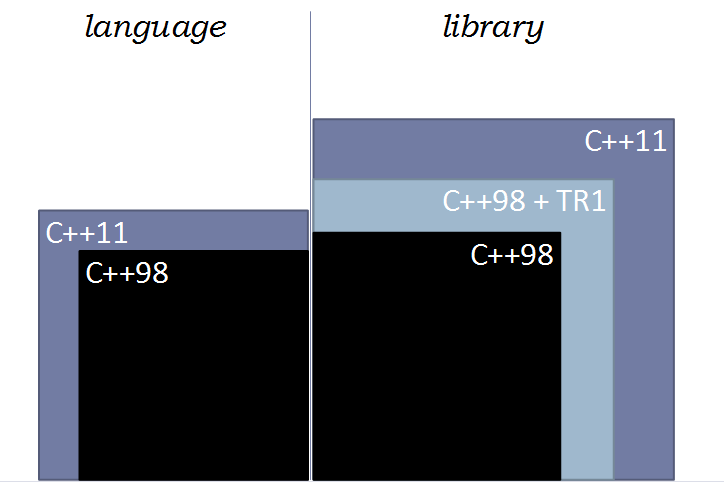
\includegraphics[height=0.7\paperheight]{cpp_libs}}
            \only<2>{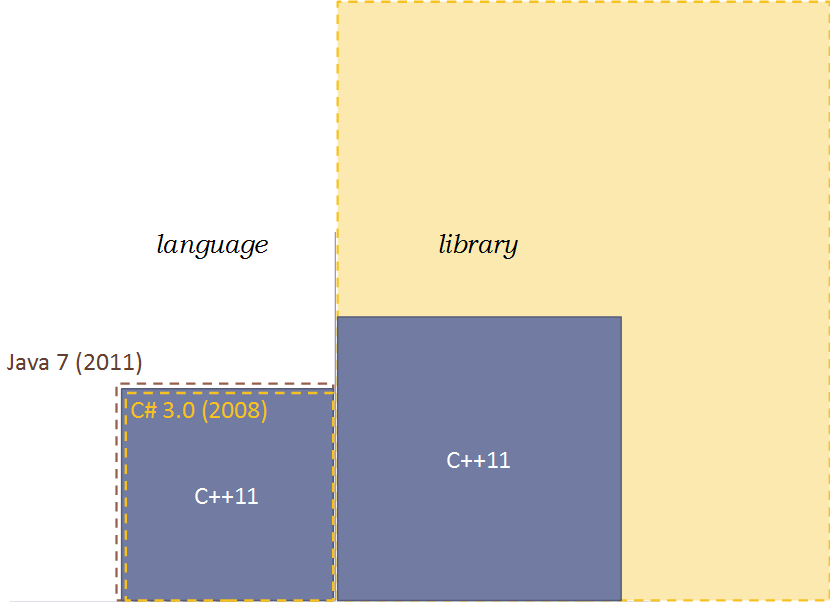
\includegraphics[height=0.85\paperheight]{cpp11_lib}}
            \only<3>{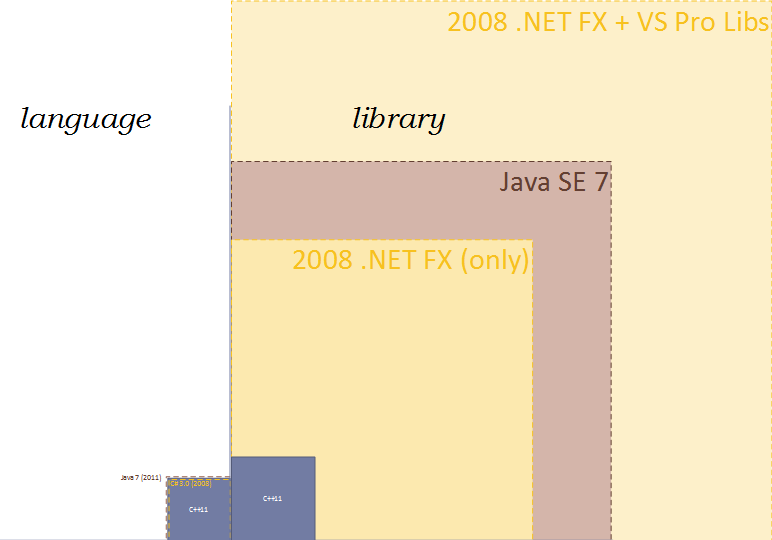
\includegraphics[height=0.8\paperheight]{cpp11_lib2}}\\
            \only<4>{\centering 
\includegraphics[height=0.8\paperheight]{bloated-jabbascript-frameworks}}
        \end{column}
    \end{columns}
}

\sectionSlide{Language popularity}{languages-popularity}{\paperwidth}{t}

\slide{What is the most popular programming language?}{
    \centering
    
\includegraphics[height=0.8\paperheight]{it-depends}
}

\slide{C++ users}{
    \begin{columns}
        \begin{column}{0.5\textwidth}
            {\small 
                \begin{table}
                    %\caption{C++ users}
                    \begin{tabular}{|l|r|}
                        \hline \textbf{Date} & \textbf{Estimated users} \\
                        \hline 
                        \hline 1979 & 1 \\
                        \hline 1980 & 16 \\
                        \hline 1981 & 38 \\
                        \hline 1982 & 85 \\
                        \hline 1983 & ??+2 \\
                        \hline 1984 & ??+50 \\
                        \hline 1985 & 500 \\
                        \hline 1986 & 2 000 \\
                        \hline 1987 & 4 000 \\
                        \hline 1988 & 15 000 \\
                        \hline 1989 & 50 000 \\
                        \hline 1990 & 150 000 \\
                        \hline 1991 & 400 000 \\
                        \hline
                    \end{tabular}
            \end{table}}        
        \end{column}
        \begin{column}{0.5\textwidth}
            \pause
            Main users:
            \itemstep{
                \item Bjarne,
                \item Bjarne's colleagues from AT\&T Bell Labs,
                \item universities,
                \item HP, IBM, AT\&T, DEC,
                \item Borland,
                \item Later: Microsoft, Apple,
                \item Now: Google, Facebook
            }
        \end{column}
    \end{columns}
}


\slide{C++ users}{
    \centering 
    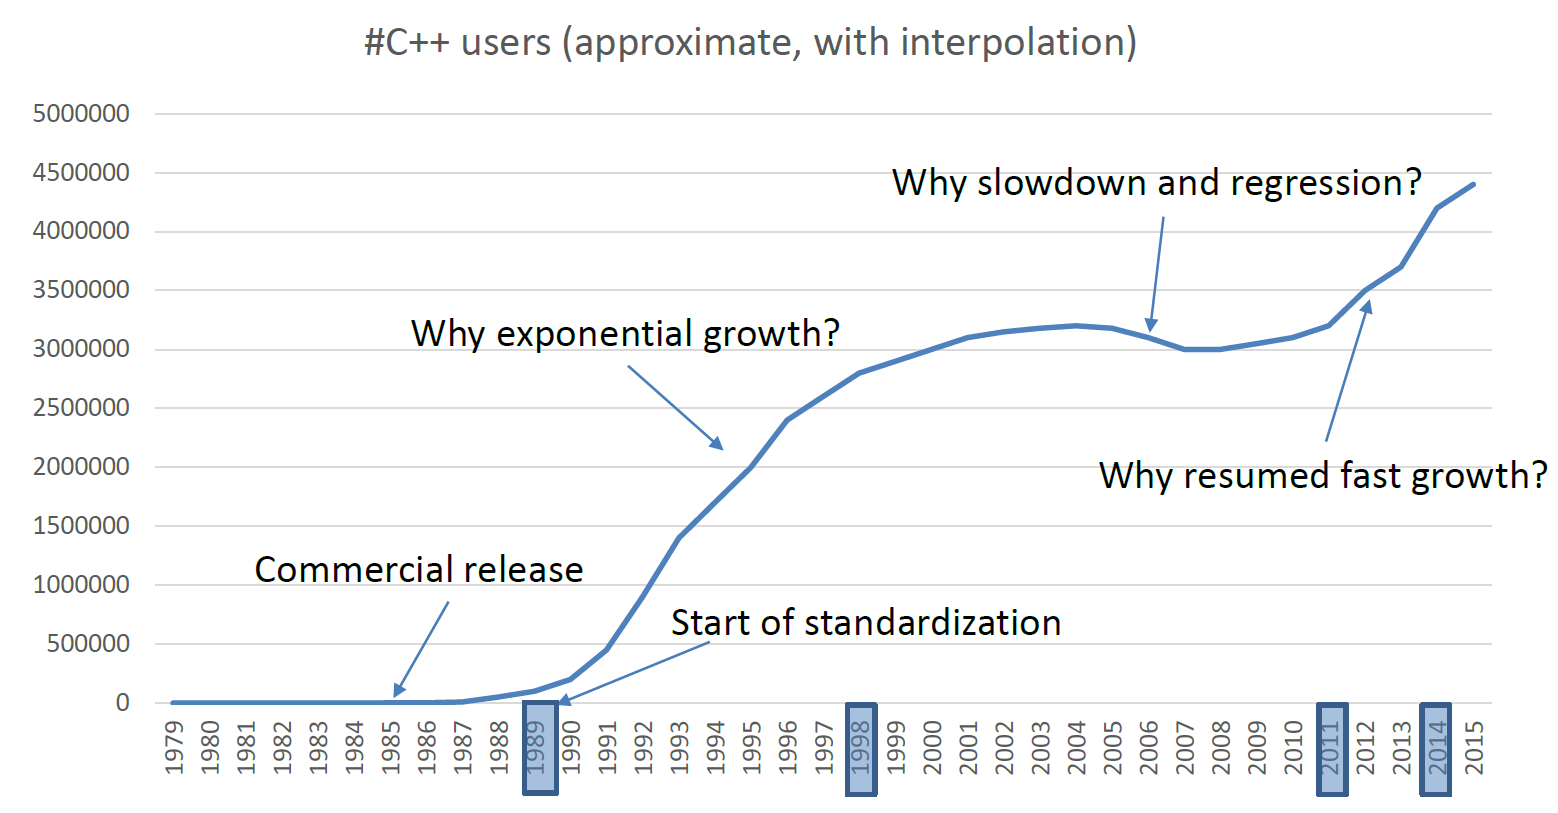
\includegraphics[height=0.8\paperheight]{cpp_users} %TODO: Loga firm na wykresie dodać
    %TODO: wyrzucić pytania, zostawić hasła
}


\slide{TIOBE - market share}{
    \only<1>{
        \begin{block}{TIOBE index}
            \textbf{The TIOBE Programming Community} index is an indicator of the popularity of programming languages. The index is updated once a month. Popular search engines such as \textbf{Google, Bing, Yahoo!, Wikipedia, Amazon, YouTube} and \textbf{Baidu} are used to calculate the ratings. Search phrase is \textbf{"language programming"} \\
            Webpage: \url{http://www.tiobe.com/tiobe-index//}
        \end{block}
    }
    \centering 
    \includegraphics<2>[height=0.7\paperheight]{tiobe-graph-grey}
    %TODO: Na dole zielona krecha C++
    \includegraphics<3>[height=0.7\paperheight]{tiobe-graph}
    \includegraphics<4>[height=0.7\paperheight]{tiobe-array} % TODO: zaznaczyć gdzie jest C++  
}


\slide{PYPL}{
    \only<1>{
        \begin{block}{PYPL index}
            \textbf{The PYPL PopularitY of Programming Language} Index is created by analyzing how often \textbf{language tutorials} are searched on Google: the more a language tutorial is searched, the more popular the language is assumed to be. It is a leading indicator. The raw data comes from \textbf{Google Trends}. \\
            Webpage: \url{http://pypl.github.io/PYPL.html}  
        \end{block}
    }
    \centering 
    \includegraphics<2>[height=0.8\paperheight]{pypl-graph-grey}
    %TODO: Lepiej opisać wykres
    \includegraphics<3>[height=0.8\paperheight]{pypl-graph}
    \includegraphics<4>[height=0.8\paperheight]{pypl-array}
}


\slide{codeeval}{
    \only<1>{
        \begin{block}{codeeval MPCL}
            \textbf{"Most Popular Coding Languages"} is based on hundreds of thousands of data points we've collected by processing over 1,200,000+ \textbf{challenge submissions on codeeval.com} in (now) 26 different programming languages. \\
            Webpage: \url{http://blog.codeeval.com/}  
        \end{block}
    }
    \centering 
    \includegraphics<2>[height=0.83\paperheight]{codeeval2016}
    \includegraphics<3>[height=0.83\paperheight]{codeeval2015}
%    \includegraphics<4>[height=0.34\paperheight]{codeeval2014}
}


\slide{langpop.corger.nl}{
    \centering
    
\includegraphics[height=0.5\paperheight]{github-logo} \vline
    
\includegraphics[height=0.5\paperheight]{stackoverflow-logo} \\
    Webpage: \url{http://langpop.corger.nl/} 
}


\imageSlide{langpop-graph} %TODO: Lepiej oznaczyć osie


\slide{Stackoverflow issues}{
    \begin{columns}
    \begin{column}{0.6\textwidth}
        \itemstep{
            \item good programmer == lazy programmer
            \item lazy programmer != good programmer
            \item good programmers do not reinvent the wheel
            \item do job once and never come back here
        }
    \end{column}
    \begin{column}{0.4\textwidth}
        \centering 
        \includegraphics<3->[height=0.8\paperheight]{copying-and-pasting-from-stack-overflow}
    \end{column}
    \end{columns}
}


\slide{C++ is not dead!}{
    \begin{columns}
    \begin{column}{0.6\textwidth}
        \begin{itemize}
            \item In the worst case C++ is on 7th place
            \item In the best case C++ is on 3rd place
            \item C++ is one of the most popular languages!
    		\item There will be next versions of C++ %TODO: przeredagować jeszcze
        \end{itemize}
    \end{column}
    \begin{column}{0.4\textwidth}
        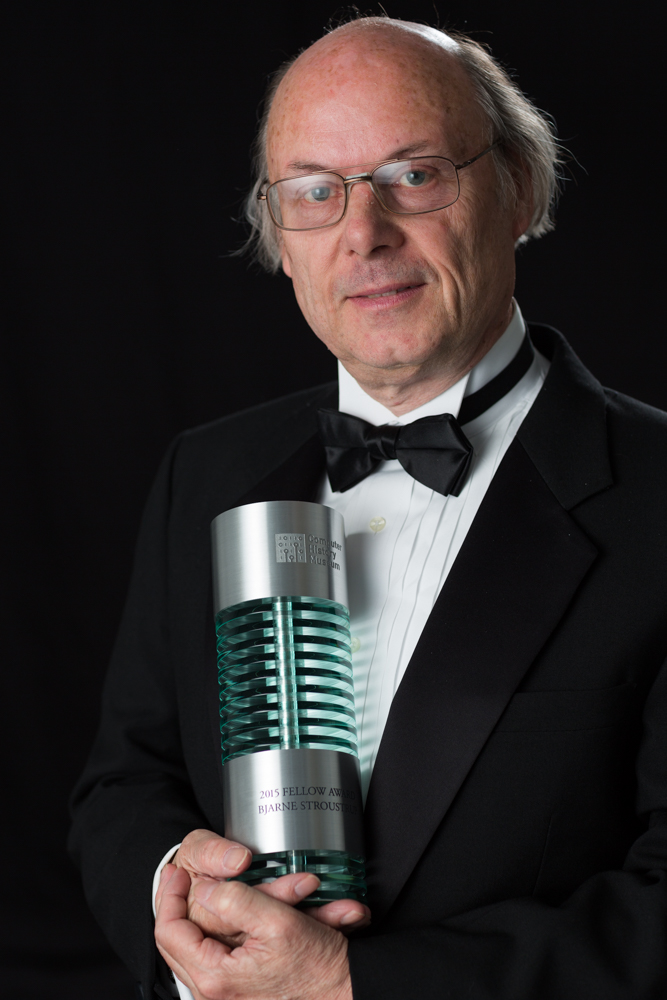
\includegraphics[height=0.8\paperheight]{bjarne-stroustrup}
    \end{column}
    \end{columns}
}


